%+++++++++++++++++++++++++++++++++++++++++++
%   Language Decision

%ENGLISH-VERSION - DEFAULT
\documentclass{acm_proc_article-sp}

%GERMAN-Version
%\documentclass{acm_proc_article-sp-german}
%+++++++++++++++++++++++++++++++++++++++++++


\usepackage{makeidx}  % allows for indexgeneration
\usepackage{graphicx}
\usepackage{tabularx}
\usepackage{amssymb}
\usepackage{amsmath}
\usepackage{color}
\usepackage{hyperref}
\usepackage[acronym]{glossaries} % Glossar und Akronyme

% folgende Zeile erzwingt URL-Umbrueche
\def\UrlBreaks{\do\/\do-}
\usepackage{tikz}
\usetikzlibrary{arrows,shapes,trees,backgrounds}

\begin{document}

\title{
	Secure Email - A Usability Study\\
	\vspace{20pt}
	\large
	\affaddr{Projet Fin d'�tudes (PFE)}\\
	\affaddr{CryptogrAphie, S�curit�, et vie Priv�e dans les Applications et R�seaux (CASPAR)}\\
	\affaddr{Supervisor: Karima Boudaoud}\\
	\affaddr{Polytech Nice Sophia Antipolis}\\
}

\numberofauthors{3} 

\author{
	Adrian Reuter\\
	\affaddr{Technische Universit�t M�nchen (TUM)}\\
	\affaddr{Email: adrian.reuter@tum.de}
	\and
	Ahmed Abdelmaksoud\\
	\affaddr{Polytech Nice Sophia Antipolis}\\
	\affaddr{Email: }
	\and
	Wadie Lemrazzeq\\
	\affaddr{Polytech Nice Sophia Antipolis}\\
	\affaddr{Email: }
}


\maketitle
%\pretolerance=150

\newacronym{ca}{CA}{Certification Authority}
\newacronym{pgp}{PGP}{Pretty Good Privacy}
\newacronym{pep}{pEp}{Pretty Easy Privacy}
\newacronym{smime}{S/MIME}{Secure Multipurpose Internet Mail Extension}
\newacronym{email}{e-mail}{electronic mail}

%++++++++++++++++++++++++++++++++
%+   ABSTRACT                   +
%++++++++++++++++++++++++++++++++
\begin{abstract} 
%++++++++++++++++++++++++++++++++
%+   ABSTRACT                   +
%++++++++++++++++++++++++++++++++

%In this paper, we describe ....
% summary of work done in this / for this paper
In a world that is becoming more digitally interconnected every day, most
webservices running in the internet critically depend on cyber security measures for preventing cyber-crime and protecting user privacy. A huge step towards more secure internet communication has been the integration of end-to-end cryptography in mobile internet messenger services such as Whatsapp or Telegram. In contrast, for securing one of the most commonly used communication channels -- the \acrlong{email} -- end-to-end encryption is only applied to approximately 5\% of email traffic. That is even though end-to-end encryption technologies for \acrshort{email}s do exist since decades, namely \acrfull{pgp} and \acrfull{smime}. Our research analyses why users hestitate to secure their \acrshort{email} communication. Particularily we investigate which usability issues exist for \acrshort{pgp}, \acrshort{smime} as well as for a fairly new technology called \acrfull{pep}. Therefore we both execute an online survey and conduct live observations in which participants actively use encryption, in order to get a precise and authentic view on usability issues.
\newline
We found that more than 60\% of \acrshort{email} users are unaware of the existance of such encryption technologies and never tried to use one. We find that above all, users 1$)$ are overwelmed with the management of public keys and 2$)$ struggle with the setup of encryption technologie in their mail software. Even though users struggle to put \acrshort{email} end-to-end encryption into practice, we experience roughly the same amout of users being aware of the importance of \acrshort{email} encryption, with 66\% rating email encryption important or even very important. Additionally we find that users are very concerned about identity theft, as 78\% want to make sure that no other person is able to write email in their name. We conclude with improvements for each of the three encryption technologies analysed, that will help to reduce usability issues and in consequence hopefully lead to a wider adoption of end-to-end \acrshort{email} encryption.
\end{abstract}

%++++++++++++++++++++++++++++++++
%+   Keywords                   +
%++++++++++++++++++++++++++++++++
\keywords{Source Routing, Source Packet Routing, Segment Routing, MPLS, SPRING, RPL, DSR, RH0} 

%++++++++++++++++++++++++++++++++
%+   Chapters                   +
%++++++++++++++++++++++++++++++++
\section{Introduction}
The most valuable information that is collected and traded in today's internet, is the personalized data of internet users. To prevent cyber-crime and to protect user privacy, almost all services running in the internet critically depend cyber security measures. Most dominantly, transport layer security (TLS) is used for securing a variety of communication protocols. Particularly when browsing the world wide web using HTTP, transport security has found wide adoption and awareness of its imperative necessity. Internet Banking, shopping on Amazon.com, accessing governmental e-services - those are just a few examples for internet use cases in which users became more and more aware of the security critical nature of these web applications, even if they might not understand the attack vectors and their risks in depth. 

A huge step towards more secure internet communication has been the integration of end-to-end cryptography in mobile internet messenger services such as Whatsapp, Signal or Telegram. In contrast, for securing one of the most commonly used communication channels - the electronic mail - end-to-end encryption is only applied by a neglectable faction \cite{secureEmail} of email users. Standardized technologies for cryptographically securing email exchanges have been available for decades. Nevertheless most users rely on unencrypted and unauthenticated email communication, often without being aware that there exist mechanisms which would mitigate the security implications that come with it. The relevance of applying end-to-end cryptography to our daily email communication can be exemplarily depicted with the following scenarios:
\begin{itemize}
	\item Protecting confidentiality \newline
	The content of an email should be kept confidential and should not be readable by someone other than the intended recipient of the email. Emails often communicate sensitive data about human or non-human assets.
	For example: Personal data, business secrets, industrial know-how, investigative journalism and almost all password-recovery routines for any web application critically depend on email exchanges.
	\item Protecting privacy \newline
	Personal information of users communicated over emails should not be processed and analyzed by any other entity than the intended recipient of the email.
	For example: Entities that can listen to internet traffic such as internet service providers, email providers themselves, analytics services should not be able to collect personal data exchanged via email, as the content was not intended to be exposed to 3rd party entities
	\item Protecting integrity \newline
	The content of an email should not be tampered with by any other entity other than the sender of an email, i.e. no other entity should be able to altering the content without the recipient being able to detect this illegitimate modification. This feature is typically provided by a digital signature.
	\item Provide authenticity and non-repudiation
	No entity should be able to impersonate another email user and write emails in his or her name. In order words, the recipient of an email should be able to trust the origin of an email; a received email should not originate from any other entity than the sender indicated to the recipient. Likewise, a sender should not be able to disclaim the content of sent mails, which provides non-repudiation for the recipient.
	For example: Information distributed via mail (e.g. agreements on deliverables, meeting appointments, conditions and contract sent within email as document in email attachments) cannot neither be changed nor denied afterwards.
	Emails are authentic and are not spoofed, severely complicating phishing attacks.
\end{itemize}
To achieve the previously mentioned security goals, two major end-to-end encryption technologies exist since decades, namely Pretty Good Privacy (PGP) \cite{rfc1991} and Secure Multipurpose Internet Mail Extensions (S/MIME) \cite{rfc2633}. A recent initiative called Pretty Easy Privacy (pEp) \cite{pEp} made efforts to simplify the usage of end-to-end cryptography in email communication for novice users. Unfortunately, those technologies are still barely deployed. According to \cite{secureEmail} more than 95\% of the overall email traffic is exchanged without end-to-end encryption.
\newline
\newline
\textbf{Our central research questions are:}
\begin{itemize}
	\item identifying why users are hesitating to use the above mentioned technologies.
	\item which usability issues exist that hinder users from securing their daily email communication using end-to-end encryption.
\end{itemize}


\section{Analysis of end-to-end Encryption Technologies for Emails}
\label{chap:analysis-encryption}

\subsection{ \acrfull{pgp} }
\label{chap:analysis-pgp}

Developed by Phil Zimmermann in 1991, \acrfull{pgp} is an encryption program that provides cryptographic privacy and authentication for data communication. \acrshort{pgp} is used for signing, encrypting, and decrypting texts, e-mails, files, directories, and whole disk partitions and to increase the security of e-mail communications. In this study we will focus only on using \acrshort{pgp} for \acrshort{email} security (\acrshort{email} encryption). It follows the OpenPGP standard for encrypting and decrypting data. Many \acrshort{email} clients provide OpenPGP-compliant \acrshort{email} security as described in RFC 3156 \cite{rfc3156}. The current specification is RFC 4880 (November 2007) \cite{rfc4880}. \acrshort{pgp} encryption uses a serial combination of hashing algorithms (SHA-1, SHA-224 / 256 / 384 / 512), data compression algorithms (zip, zlib, and bzip2), symmetric encryption algorithms (3DES, AES-128 / 192 / 256, CAST5, IDEA) and finally asymmetric encryption algorithms (ElGamal, RSA (MUST NOT <1024 bits)).

In \acrshort{pgp}, one-off key is generated randomly, which is known as the session key. The session key encrypts the message, which is the bulk of the data that needs to be sent. This type of encryption is relatively efficient, but it has a problem of sharing the session key with your recipient because without the key your recipient will only see the ciphertext. \acrshort{pgp} solves this problem with public-key cryptography, also known as asymmetric cryptography. In this kind of encryption there are two keys: a public key and a private one. The public key of your potential correspondent can be found by searching through key servers or by asking the person directly. Moreover, each public key is bound to an \acrshort{email} address and has a unique fingerprint which can be used to get the right corresponding public key \cite{pgpWiki}. In \acrshort{pgp}, public-key encryption isn't used to encrypt the message, just the one-off session key that was generated to encrypt it. It would take too long and use a larger amount of computational resources. Since the body of the message usually contains the bulk of the data, \acrshort{pgp} uses the more economical symmetric-key encryption for this. It reserves the lumbering public-key encryption for the session key, making the whole process more efficient. Our written signatures are frequently used to verify that we are who we say we are. They are far from foolproof, but they are still a useful way of preventing fraud.
\newline
Digital signatures are similar, using public-key cryptography to authenticate that the data comes from the source it claims to and that it has not been tampered with. Digital signatures work by using an algorithm to combine the sender's private key with the data that they are authenticating. The plaintext of the message is fed through a hash function, which is an algorithm that transforms inputs into a fixed-size block of data, called a message digest. The message digest is then encrypted with the sender's private key. This encrypted message digestis what is known as the digital signature \cite{pgpTech}. In \acrshort{pgp}, the digital signature is sent alongside the message body (which can either be encrypted or in plaintext). When someone receives a digitally signed \acrfull{email}, they can check its authenticity and integrity by using the public key of the sender. First, a hash function is used on the message that was received and this gives the message digest of the email in its current form \cite{pgpTech}. The next step is to calculate the original message digest from the digital signature that was sent. The sender's public key is used to
decrypt the digital signature, and this gives the message digest exactly as it was when it was signed by the sender. The final step is to compare the message digest from the email they received to the message digest that they derived from the digital signature. If the message has been altered, then the message digests will be completely different, and the recipient will know that there is a problem with the message. If the two message digests are not identical, there are three likely culprits \cite{pgpTech}:
\begin{itemize}
	\item The public key used to decrypt the digital signature was not linked to the private key that was used to encrypt it. This means that the sender may not be who they say they are.
	\item The digital signature may be fake.
	\item The message has been changed since it was signed.
\end{itemize}
In addition to all these security measures, another important factor is the emails attachments. PGP can also be used to encrypt your attachments. There are a two of ways to do this:
\begin{itemize}
	\item One approach to encrypt an email with \acrshort{pgp} is to encrypt everything separately. This means that the message body and attachments are individually encrypted and signed. It’s called PGP/Inline \cite{pgpAttachements}.
	\item A newer approach is PGP/MIME, which - in contrast to PGP/Inline - encrypts and signs the message as a whole, including attachments \cite{pgpAttachements}.
\end{itemize}
Finally, \acrshort{pgp} relies on the concept of web of trust to establish trust between the users. it is critical that the public key used to send messages to someone or some entity actually does 'belong' to the intended recipient [5]. Simply downloading a public key from somewhere is not a reliable assurance of that association. The web of trust grew as a way of vetting that each PGP public key and user are really connected to the person or organization that they are said to represent. The web of a trust connects the real-life entity with their public key by using a third party to sign the user’s PGP public-key and it does it all without a central authority that can collapse or be corrupted [6]. If a user knows another PGP user personally, he can confirm that their public key is linked to their actual identity. He can put his trust in them and digitally sign his public-key, which shows that at least one person vouches for his identity. Then, he can also do the same. Over time, this builds an interconnected web of trust, with lots of people vouching for each other with digital signatures that verify their ownership of a public key.

In conclusion, \acrshort{pgp} encryption leverages a range of techniques to provide secure and private email communications. These include compression, public-key encryption, symmetric encryption, digital signatures, and the web of trust. Together, these allow its users to send encrypted messages in an efficient manner. It also let them check whether a message is authentic and has not been altered. The OpenPGP standard was formed so that everyone could use it for free, helping to make it the most widespread form of email encryption and protect the privacy of email users.
\subsection{\acrfull{smime}}
\label{chap:analysis-smime}

With the increase of power in terms of computation and networking capability, people's need for using non-textual objects such as image, audio, and video in emails became a fair demand. To support diversity of content, multipart message structure, and non-English text, the \acrfull{mime} was proposed in 1993 \cite{rfc1521}. \acrfull{smime} is an enhancement of \acrshort{mime} to provide cryptographic security for \acrshort{mime} based emails \cite{rfc1521}. %To better understand \acrshort{smime}, let us first take look at \acrshort{mime}.
\acrshort{smime} adds some additional content types to the \acrshort{mime} to provide security features. The current \acrshort{smime} version 3.2 obsoletes all earlier versions. However, most implementations still bear version 3.1 features for digital signature processing. Today, popular email clients such as MS Outlook 2013, MS Outlook 2016, Mozilla Thunderbird, Apple Mail support \acrshort{smime} enabled messages.
%\acrshort{smime} version 3.2 is defined by the following five major specifications.
%\begin{itemize}
%\item Cryptographic Message Syntax (RFC 4853 \cite{rfc4853})
%\item Cryptographic Message Syntax (CMS) Algorithms (RFC 3370 %\cite{rfc3370})
%\item Diffie-Hellman Key Agreement Method (RFC 2631 \cite{rfc2631})
%\item S/MIME Version 3.2 Certificate Handling (RFC 5750 \cite{rfc5750})
%\item S/MIME Version 3.2 Message Specification (RFC 5751 \cite{rfc5751})
%\item Enhanced Security Services for S/MIME (RFC 2634 \cite{rfc2634})
%\end{itemize}
\newline
\newline
\textbf{Cryptographic Message Syntax (CMS)}
\newline
To define how security features, such as confidentiality or integrity, can be added to \acrshort{mime} content types, \acrshort{smime} defines Cryptographic Message Syntax (CMS). The syntax in each case defines the exact encoding scheme for each content type. Discussed below are the different types of messages and different sub-types that are created from these messages \cite{PKCS-7}.
\begin{itemize}
\item Data Content Type is an arbitrary string.  The object created is called "Data".
\item Digested-Data Content Type is used to provide integrity for the message. The result is typically used as the content for the enveloped-data content type. The encoded result is an object called "digested-data". The process of creating "digested-data" involves the following two steps
\begin{enumerate}
\item Using the hash algorithm of the user's choice a message digest is created from the content.
\item The message digest, the algorithm, and the content are added together to create the "digested-data" object.
\end{enumerate}
\item Signed Data Content Type provides authenticity and integrity of data. It contains any type and zero or more signature values. The encoded result is an object called "signed-data". A signed data message can only be viewed by the recipient of with \acrshort{smime} capability. The following are the steps in the process.
\begin{enumerate}
\item For each signer, a message digest is created from the content using the specific hash algorithm chosen by the signer.
\item Each message digest is signed by the signer with his or her private key.
\item The content, signature values, certificates, and the algorithms are then collected to create the "signed-data".
\end{enumerate}
\item Enveloped-Data Content Type is used to provide privacy for the message. It contains encrypted content of any type, and zero or more encrypted keys and certificates. The encoded result is an object called "enveloped-data". The steps involved in the process is are as follows
\begin{enumerate}
\item A pseudo-random session key is created for the symmetric-key algorithm to be used to encrypt the content.
\item The content is encrypted using the defined algorithm and created session key.
\item For each recipient, a copy of the session key is encrypted with the public key of the recipient.
\item The encrypted contents, encrypted session keys, algorithm used, and certificates are encoded using Radix-64.
\end{enumerate}
\end{itemize}
\textbf{Cryptographic Algorithms}
\newline
\acrshort{smime} specifies several cryptographic algorithms for use. The term "must" indicate absolute requirement, and the term "should" imply recommendation only. \acrshort{smime} recommends using SHA-256 as hash function for creating message digests. For content encryption RSA is recommended.
\newline
\newline
\textbf{Key Management and Certification}
\newline
\acrshort{smime} relies on the X.509 \acrfull{pki} to exchange and validate the public keys of other \acrshort{email} users. Therefore, each \acrshort{smime} user has to get a X.509 public key certificate signed by a trustworthy \acrfull{ca}. This digital certificate is always added to any outgoing \acrshort{email}. When an \acrshort{email} user receives an \acrshort{email} secured via \acrshort{smime}, he can always extract the sender's public key and validate it using the attached certificate. The certificate is trustworthy as it was signed by a trusted \acrlong{ca}.
\subsection{\acrlong{pep}}
\label{chap:analysis-pep}
\acrfull{pep} is an initiative which aims to simplify end-to-end communication security. It is developed by two entities:
\begin{enumerate}
	\item \acrshort{pep} Foundation, a non-profit organization based in Switzerland, owning trademarks and the pEp engine
	\item \acrshort{pep} Security AG, a company based in Switzerland and Luxembourg, developing commercial \acrshort{pep} app and plugin implementations
\end{enumerate}
The principle design goal of \acrshort{pep} is being easy-to-install and easy-to-use. \acrshort{pep} is strongly based on OpenPGP and its message format, but introduces several enhancements and new concepts in favor of usability and ease-to-use. The major conceptual improvement consists of depending less on user interaction and automatizing procedures, as well as moving forward to a security by
default instead of a security by opt-in philosophy. Up to point of this paper, there exist three major implementations of \acrshort{pep} that can already be
purchased and downloaded for usage: a Microsoft Outlook Plugin, a Mozilla Thunderbird plugin and a Google Android mobile app. Furthermore there is an Apple iOS mobile app announced to be in development and released soon \cite{15}.
\newline
\newline
\textbf{Automatic Key Management}\newline
To achieve its primary design goal, \acrshort{pep} is designed to work without prior configuration by the user and to provide encryption by default and without user interaction \cite{15}. The own \acrshort{pgp} key pair is automatically generated in background upon first usage of \acrshort{pep}, or imported automatically if the user previously used \acrshort{pgp} and already has a key pair on his system. Key pairs generated by \acrshort{pep} are RSA 4096 key pairs by default. If in the latter case an existing \acrshort{pgp} key pair has less than 2048 bit length, a new key pair is generated instead of using the old key, such that the \acrshort{pep} security level does not fall below the commonly recommended RSA key length of 2048 bit for todays usage \cite{16}.
The own public key is always attached as file \emph{pEpkey.asc} to each outgoing email, and consequently the public keys of other pEp users are received respectively by incoming mails \cite{16}. Those public keys extracted from incoming mails are imported automatically into \acrshort{pep}. Using this key management approach, \acrshort{pep} does not depend on any centralized infrastructure such as key servers (as for \acrshort{pgp}) or a \acrshort{pki} based on external certification authorities (as for \acrshort{smime}). As consequence, the manual key import by the user as it is known for \acrshort{pgp} is circumvented and key management is fully automated. Encryption is applied by default once received the communication partner's public key, i.e. the user does not have to opt-in encryption manually.
\newline
\newline
\textbf{\acrshort{pep} Handshake}\newline
A careful reader will recognize that the automatic key import mechanism explained above is vulnerable to a potential \acrfull{mitm} attacker: He could replace the legitimate key in the mail attachment with his own key file. This fraudulent key would then be imported automatically without further verification, and the attacker could decrypt all mails sent to the victim whose key was replaced.
\newline
To mitigate this risk, pEp let's its users do a so-called \acrshort{pep} handshake: Once both \acrshort{pep} users received an email from the respective other user and thus having received its public key, \acrshort{pep} offers an option to verify the fingerprint of the received key. This is done by comparing so-called trustwords, which are shown on the screens of both users. These trustwords have to be compared via an out-of-band process, e.g. a phone call or any other secure instant messenger. Trustwords are 16-bit mappings between natural language words (e.g. english language) and the bitwise XOR of the own public key and the one of the communication partner \cite{17}. If the trustwords shown to both users are equivalent, the received key is verified and can be trusted, with no \acrshort{mitm}-attacker being present. The users can select to either trust or mistrust the other party's public key according to the result of the trustword
comparison. To support compatibility with \acrshort{pgp} users, the key fingerprint is also shown next to the trustwords, so that pEp users can always fall back to directly comparing fingerprints with non-pEp users \cite{19}.
\newline
\newline
\textbf{Enhanced Security Status Transparency}\newline
\acrshort{pep} strives to make the security status of each individual communication channel (i.e. an email exchange with a certain recipient) more transparent and easy to assess for users. It does so by using a standardized color scheme which represents the security status of a channel. The status of no cryptographical end-to-end protection being applied is represented by grey colored icon, displayed by a visually dominant icon in the graphical interface when writing a new mail. This status corresponds to email communication with a recipient that do not use \acrshort{pep}, or to the very first mail sent to another \acrshort{pep} user \cite{15}. Once received the public key of the recipient as \acrshort{email} attachment, future \acrshort{email}s to that recipient will be sent encrypted and integrity protected, represented by a yellow colored icon. After two users successfully performed a handshake and chose to trust the other party's public
key, this status is represented by a green icon \cite{15}. In case there is a trustword mismatch (a potential \acrshort{mitm}-attacker in place) and the users choose to mistrust the received key, this status is represented by a red colored icon. It is important to mention that the step of mistrusting a public
key is non-reversible and can't no be undone other than deinstalling the \acrshort{pep} instance -- which evidently would also delete any positive handshake results \cite{18}.



\section{Conclusion}
With our project, we identified the most frequent usability issues that users face when protecting their email communication using \acrlong{pgp} (\acrshort{pgp}), \acrlong{smime} (\acrshort{smime}) or \acrlong{pep} (\acrshort{pep}). First, we did a technical analysis of those three technologies, elaborating on trust establishment, key exchange, cryptographic algorithms and provided security features. 
Secondly we prepared and launched an online survey, aiming for a broad audience to collect a maximum feedback. The survey does not only identify the usability issues of each technology, but also assesses the general impression of our audience towards the importance of email encryption. Third, we conducted live observations in which participants were to install, configure and use either \acrshort{pgp}, \acrshort{smime} or \acrshort{pep} in presence of a team member that observed the participant testing the technologies and that provided support in case the participant encountered difficulties.
Our three fold approach gave us both, an overall view on the awareness of the email users as well as a detailed view on the causes for which users are hesitating to use the mentioned technologies. The overall impression we received from the online survey showed us that the email users are aware of the importance of email encryption with 32\% saying it's very important. Additionally, users are very concerned about identity theft, as 78\% of the participants want to make sure that no other person is able to write email using their name and 80\% of the participants want to be sure that the content of their mail isn't changed by someone else while being transferred to the recipient. It shows that for many users, signing emails is more important than encrypting them. For the usability issues we found, we propose some sample improvements that we suppose will make it easier for the users to apply \acrshort{pgp}, S/MIME or pEp in their email communication.
\newline
We present the improvement suggestions by technology:
\vspace{-5pt}
\begin{itemize}
	\item \textbf{Improvements for \acrshort{pgp}:}\newline
	We found out that on all tested platforms, users are restricted to the search for the recipient key only at one key server at a time, which makes importing the recipient key the major obstacle when using \acrshort{pgp}. Thus, we suggest to fix this issue by letting implementations search for the recipient key on all available key-servers at a time, without the user needing to manually adjust the key server for key import
	\item \textbf{Improvements for \acrshort{smime}}\newline
	We suggest Certification Authorities to send further information on how to import the certificate into the most frequently used email programs, alongside the email which contains the requested digital certificate. Also, we suggest to integrate \acrshort{smime} support into webmail plugins, as webmail nowadays is used more commonly than dedicated desktop applications.
	\item \textbf{Improvements for \acrshort{pep}}\newline
	We suggest \acrshort{pep} implementations to add further explanation on what to do with the trustwords displayed to the users during handshake. We furthermore advise to briefly explain the \acrshort{pep} color scheme that represents the security status of a communication channel to the user.
	Moreover we criticize the design choice of not being able to do a new handshake with a user whose public key was previously mistrusted. As a trustword mismatch can too easily occur due to a different language selection of the trustword dictionary on side of both users.	
\end{itemize}

\section{Examplary Content}
\label{chap:spring}
In order to advance the research and standardization of a flexible and universal source routing mechanism, the Internet Engineering Task Force (IETF) has formed a working group (WG) in 2013. This WG, called \emph{Source Packet Routing in Networking (SPRING)}, is chartered to identify source routing use cases as well as defining the requirements and mechanisms for implementing, deploying and administrating source routing enabled networks \cite{springcharter}. The working group yet developed a new source routing mechanism called \emph{segment routing} \cite{spring-sr-10}, which is discussed in section \ref{sec:spring-sr}. It further introduced two implementational approaches \cite{spring-ipv6,spring-mpls}, which will be discussed in section \ref{sec:spring-mpls} and \ref{sec:spring-ipv6}. The working group is currently preparing their final document revisions for a technical review and adoption to IETF standards track \cite{springstatus}.

\subsection{Segment Routing}
\label{sec:spring-sr}
Segment routing is a new source routing mechanism developed by the IETF SPRING working group. It is based on so-called \emph{segments} \cite{spring-sr-10}. The SPRING architecture \cite{spring-sr-10} defines that a segment represents \emph{"an instruction a node executes on the incoming packet (e.g.: forward packet according to shortest path to destination, or, forward packet through a specific interface, or, deliver the packet to a given application/service instance)"}. A segment and its associated \emph{Segment Identifier (SID)} is advertised within the segment routing domain with the help of the Interior Gateway Protocol (IGP) in use. Therefore the SPRING working group has defined extensions for the IGP protocols OSPF \cite{spring-ospf}, OSPFv3 \cite{spring-ospfv3} and IS-IS \cite{spring-isis}. With the help of these extensions, those protocols are able to carry the necessary segment routing signaling information. Segment routing introduces three major types of segments \cite{salsano2015pmsr,spring-sr-10}:
\begin{itemize}
	\item IGP-Prefix Segments
	\item IGP-Node Segments
	\item IGP-Adjacency Segments
\end{itemize}
Each of these segment types are discussed in the following sections. The term \emph{ingress node} identifies the node at which a packet enters the segment routing domain, whereas \emph{egress node} identifies the node at which a packet exits the segment routing domain.

\subsubsection{IGP-Node Segment}
\label{sec:nodal-segment}
An IGP-node segment has global scope and thus is identified by a globally unique SID. Each node is assigned a SID and advertises its nodal segment via the IGP protocol \cite{packet-pushers-sr-intro}. Global scope in this context means that all nodes within a segment routing domain add an entry in their Forwarding Information Base for the instruction associated with that segment \cite{cisco-whitepaper}. The node identified by the node-SID is always reached by the shortest path, which is determined by the IGP algorithm \cite{spring-sr-10}. That means an ingress node can impose a source route to a packet by specifying another node to be traversed by prepending the correspondent node-SID to that packet.
\newline
\newline
Figure \ref{fig:node-segment} shows an exemplary scenario: Node R advertised its node-SID $70$ to all other nodes within the domain. Node S can instruct incoming packets to traverse node R by prepending the node-SID $70$ to it. Hence the packet will be either forwarded via the path \{S,A,B,R\} or \{S,C,D,R\}, depending on which of both paths have been investigated as the shortest path. Intermediate nodes do not change the prepended SID, thus symbolically swapping it from $70$ to $70$, except for the last node. The last node on the path towards R is directly connected to R and thereby can remove the SID as this information is not needed anymore \cite{packet-pushers-sr-intro}.

\begin{figure}%[h]
	\centering
	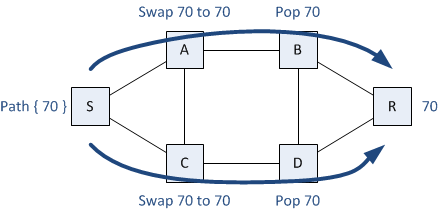
\includegraphics[width=0.95\linewidth]{figures/node-segment-2.png}
	\caption{Node Segments \cite{packet-pushers-sr-intro}}
	\label{fig:node-segment}
\end{figure}

%\bibliographystyle{abbrv}
\bibliographystyle{ieeetr}
%++++++++++++++++++++++++++++++++++++++++
%+   Refernces - .bib-File version  +
%++++++++++++++++++++++++++++++++++++++++
\bibliography{ref,rfc}

\end{document}

%++++++++++++++++++++++++++++++++
%+    Figure                    +
%++++++++++++++++++++++++++++++++

%\begin{figure}[h]
%	\centering
%	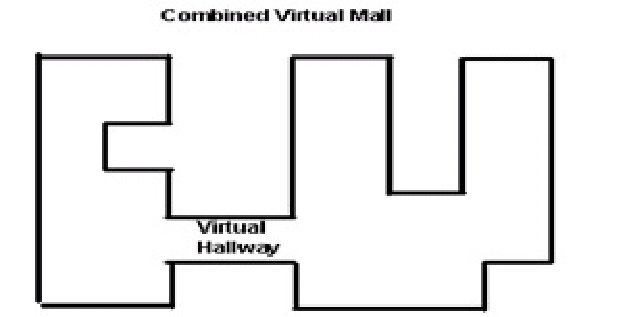
\includegraphics[width=0.95\linewidth]{graphik}
%	\caption{Graphic in b/w as .pdf}
%	\label{fig:graphik}
%\end{figure}


%++++++++++++++++++++++++++++++++
%+    Table                     +
%++++++++++++++++++++++++++++++++

%\begin{table}
%\centering
%\caption{Frequency of Special Characters}
%\begin{tabular}{|c|c|l|} \hline
%Non-English or Math&Frequency&Comments\\ \hline
%\O & 1 in 1,000& For Swedish names\\ \hline
%$\pi$ & 1 in 5& Common in math\\ \hline
%\$ & 4 in 5 & Used in business\\ \hline
%$\Psi^2_1$ & 1 in 40,000& Unexplained usage\\
%\hline\end{tabular}
%\end{table}
%
%If due to some reason the written line makes no normal 
%line-break (can be seen in the pdf.) just type /linebreak 
%in front of the corresponding word and as a consequence the 
%line-break will be done.